\documentclass[12pt]{extarticle}
\usepackage{geometry}
\geometry{
a4paper,
total={170mm,257mm},
left=20mm,
top=20mm,
headheight=12pt
}

\usepackage[parfill]{parskip} % Activate to begin paragraphs with an empty line rather than an indent
\usepackage{graphicx} % Use pdf, png, jpg, or eps§ with pdflatex; use eps in DVI mode
% TeX will automatically convert eps --> pdf in pdflatex
\graphicspath{ {./Figures/} }
\usepackage{subcaption}
\usepackage{float}

\usepackage{amssymb,amsmath,amsthm}
\usepackage{commath}
\usepackage{longtable}
\usepackage[hyphens]{url}
\usepackage[dvipsnames]{xcolor}
\usepackage[unicode=true,colorlinks=true,urlcolor=CadetBlue,citecolor=black,linkcolor=black]{hyperref}
\PassOptionsToPackage{hyphens}{url} % url is loaded by hyperref
\usepackage{authblk}
      
%SetFonts
% newtxtext+newtxmath
\usepackage{newtxtext} %loads helv for ss, txtt for tt
\usepackage{amsmath}
\usepackage[bigdelims]{newtxmath}
\usepackage[T1]{fontenc}
\usepackage{textcomp}
%SetFonts

% less space before sections 
% \@startsection {NAME}{LEVEL}{INDENT}{BEFORESKIP}{AFTERSKIP}{STYLE} 
%            optional * [ALTHEADING]{HEADING} 
\makeatletter
 \renewcommand\section{\@startsection {section}{1}{\z@}%
     {-2.5ex \@plus -1ex \@minus -.2ex}%
     {1.3ex \@plus.2ex}%
    {\Large\bfseries}}
    
% Species names
%% Meta-Command for defining new species macros
\usepackage{xspace}

\newcommand{\species}[3]{%
  \newcommand{#1}{\gdef#1{\textit{#3}\xspace}\textit{#2}\xspace}}
  
\species{\yeast}{Saccharomyces cerevisiae}{S.~cerevisiae}
\species{\calbicans}{Candida albicans}{C.~albicans}
\species{\cneoformans}{Cryptococcus neoformans}{C.~neoformans}

% Yoav & Lee commands
\newcommand*{\tr}{^\intercal}
\let\vec\mathbf
\newcommand{\matrx}[1]{{\left[ \stackrel{}{#1}\right]}}
\newcommand{\diag}[1]{\mbox{diag}\matrx{#1}}
\newcommand{\goesto}{\rightarrow}
\newcommand{\dspfrac}[2]{\frac{\displaystyle #1}{\displaystyle #2} }
\newtheorem{theorem}{Theorem}
\newtheorem{corollary}{Corollary}
\newtheorem{lemma}{Lemma}
\newtheorem{remark}{Remark}
\newtheorem{result}{Result}
\renewcommand\qedsymbol{} % no square at end of proof
\newcommand{\cl}{\mathbf{L}}
\newcommand{\cj}{\mathbf{J}}
\newcommand{\ci}{I}

% NatBib
\usepackage[round,colon]{natbib}

% Title page
\title{Cultural Transmission Can Explain the Evolution of Cooperative Behavior}

% Authors
\renewcommand\Affilfont{\small}

\author[1]{Dor Cohen}
\author[2]{Ohad Lewin-Epstein}
\author[3]{Marcus W. Feldman}
\author[a,*]{Yoav Ram}

\affil[1]{School of Computer Sciences, IDC Herzliya, Herzliya, Israel}
\affil[2]{School of Plant Sciences and Food Security, Tel Aviv University, Tel Aviv, Israel}
\affil[3]{Department of Biology, Stanford University, Stanford, CA}
\affil[*]{Corresponding author: yoav@yoavram.com}

\date{\today}

\begin{document}
\maketitle

% Abstract
%\begin{abstract}
%\end{abstract}

\pagebreak

% Introduction
\section*{Introduction}
Cooperative behavior can harm an individual's fitness and increase the fitness of its conspecifics or competitors~\citep{axelrod1981evolution}.
Nevertheless, cooperative behavior appears to occur in many non-human animals~\citep{dugatkin1997cooperation}, for example rats~\citep{rice1962altruism} and birds~\citep{krams2008experimental}.
Evolution of cooperative behavior remains  an important  conundrum in evolutionary biology.
\\
Cultural evolution is an evolutionary theory of individual and group-level change in beliefs, behaviors, and norms \citep{cavalli1981cultural}.
Culture has significant impact on the behavior of humans~\citep{ihara2004cultural,jeong2018bronze} as well as non-human animals~\citep{bonner2018evolution}.
Cultural transmission allows an individual to acquire attitudes and behavioral traits from other individuals in its social group through imitation, learning, or other modes of communication \citep{cavalli1981cultural,richerson2008not}.
Here we attempt to determine to what extent cultural transmission can explain the evolution of cooperative behavior.

% subsection
\subsection*{Theories for evolution of cooperation}
Three major theories have been proposed to explain the evolution of cooperative behavior.

\paragraph{Kin selection theory} posits that natural selection can favor cooperation between related individuals. The importance of relatedness to the evolution of cooperation and altruism was shown by~\citet{hamilton1964genetical}. According to Hamilton,  an allele that determines altruistic behavior should increase in frequency when  the reproductive cost to the actor that cooperates, $c$, is less than the benefit to the recipient, $b$, times the genetic relatedness between the recipient and the actor, $r$.
This is also known as Hamilton's Rule:

\begin{equation} \label{eq:hamilton_rule}
c < b \cdot r.
\end{equation}

There is an ongoing debate about to what extent kin selection explains evolution of cooperation and altruism.
It has been suggested that kin selection can explain the cooperative behavior of worker castes of eusocial insects like the honey bee.
The most significant argument against kin selection is that in some cases cooperation among unrelated individuals appears to have evolved~\citep{wilson2005kin}. This makes Hamilton's rule incomplete according to \citet{wilson2005kin}, although \citet{foster2006kin} reject this claim and argue that altruism cannot evolve without relatedness. They refer  to Hamilton, who claimed that relatedness can arise without recent common ancestry. %MWF: How?
\citet{wilson2005kin} also criticizes kin selection on the grounds that environmental or ecological factors are probably more important than relatedness in determining social actions. Although \citet{foster2006kin} argue that kin selection does not ignore ecology. Hamilton's rule suggests
that environmental factors causing a high benefit-to-cost ratio will favor cooperation.

\paragraph{Reciprocity} entails that repeated interactions or individual recognition are key components of the evolution of cooperation. In \emph{direct reciprocity} there are repeated encounters between the same two individuals, where at every encounter, each player has a choice between cooperation and defection: if I cooperate now, you may cooperate later. Hence, it may pay off to cooperate.
This game-theoretic framework, known as the repeated Prisoner's Dilemma, 
%A well known strategy to play this game is called  'tit-for-tat'. This strategy always starts with a cooperation, then it does whatever the other player has done in the previous round: a cooperation for a cooperation, a defection for a defection. There a unlimited number of possible strategies to play this game. However, 
can only lead to the evolution of cooperation if the cost is less than the benefit $b$ times the probability of another encounter between the same two individuals, $w$, 
%MWF: Referencess?

\begin{equation} \label{eq:reciprocity}
c < b \cdot w.
\end{equation}

Direct reciprocity assumes that both players are in a position to cooperate, but it can not explain cooperation in asymmetric interactions such as human philanthropy.  

\paragraph{Indirect reciprocity} has also been suggested as an explanation of this behavior.
\citet{nowak2006five} claims that direct reciprocity is like a barter economy based on the immediate exchange of goods, while indirect reciprocity resembles the invention of money. 
%MWF: More refs
The money that ``fuels the engines'' of indirect reciprocity is reputation. 
However, reciprocity assumes repeated interactions and therefore has difficulty in explaining the evolution of cooperation if  interactions are not repeated. 

\paragraph{Group selection theory} posits that cooperation is favored because it imparts an advantage to the whole group, if selection acts at the group level in addition to the individual level. A common model for group selection divides the population into groups in which there are cooperators that help  other group members and defectors that do not.  % TODO add reference
Individuals reproduce proportionally to their fitness, and offspring are added to the same group as their parents.
If a group reaches a certain size it can split to two groups, so groups that grow faster will split more often.
Groups with cooperators  grow faster than groups without cooperators, and
cooperation can evolve in this model when the cost $c$ is less than the benefit $b$ times the ratio between the  the number of groups $m$ and the sum of $m$ and the maximum group size $n$,

\begin{equation} \label{eq:groupselection}
c < b \cdot \frac{m}{m+n} .
\end{equation}

Group selection has been criticized by biologists who advocate a gene-centered view of evolution. Group selection has also been criticized because a trait such as cooperation evolves in the total population. For cooperation to take over the population it must have higher fitness, while under group selection the fitness of cooperators at the individual level is lower. Thus a trait with a lower fitness taking over the population is a contradiction. \citet{eldakar2011eight} reject this argument claiming that it is a tautology and does not qualify as an argument against group selection. The distinction between individual and group selection requires a comparison of fitness differentials within and between groups in a multi-group population, and when a trait  evolves by group selection, despite having lower fitness within a group, that group might have higher average fitness in competition with other groups, all things considered. 

\paragraph{}
All the above theories assume that cooperation is genetically determined, which raises the question, is it possible that cooperation is determined by non-genetic factors? \citet{feldman1985gene} introduced the first model for the evolution of altruism by cultural transmission. They showed that under vertical (parent-to-offspring) cultural transmission, Hamilton's rule does not govern the evolution of parent-to-offspring or sib-to-sib altruism.
Recent work by \citet{lewin2017microbes} also sheds some light on this question. 
They hypothesise that microbes that manipulate their hosts to act altruistically can be favored by selection, and may play a role in the widespread occurrence of cooperative behavior. Indeed, it has been shown that microbes can mediate behavioral changes in their hosts~\citep{poulin2010parasite,dobson1988population}. Therefore, natural selection on microbes may favor manipulation of the host so that it cooperates with others. Microbes can be transmitted \emph{horizontally} from one host to another during host interactions, and following horizontal transfer, the recipient host may carry microbes that are closely related to the microbes of the donor host, even when the two hosts are (genetically) unrelated~\citep{lewin2017microbes}. Microbes can also be transferred vertically, from parent to offspring, and % yr: cite 10.1126/science.aat7164
a microbe that induces its host to cooperate with another host and thereby increases the latter's fitness will  increase the vertical transmission of the microbes of the receiving individual. Kin selection among microbes could therefore favor microbes that induce cooperative behavior in their hosts, thereby increasing the transmission of their microbial kin.
%\\While the hypothesis that microbes could manipulate their hosts to act altruistically is mathematically feasible~\citep{lewin2017microbes}, there are still no empirical evidence of whether microbes indeed mediate altruistic behavior of their hosts.

% subsection
\subsection*{Cultural evolution of cooperation}
\citet{lewin2017microbes} have demonstrated that \emph{non-vertical transmission} can help to explain the evolution of cooperative behavior. 
Non-vertical transmission may be either a horizontal or oblique: horizontal transmission occurs between individuals from the same generation, while oblique transmission occurs from an adult to an offspring. 
Evolution under either of these transmission models  can be be more rapid than under pure vertical transmission~\citep{cavalli1981cultural,ram2018evolution}. % (yr: not sure that this is a good reference)

Here we suggest a model in which behavioral changes are mediated by cultural transmission that can occur during social interaction. For example, if an individual interacts with a cooperative individual, it might learn that cooperation is a positive behavior and will cooperate in the future. Some of the analysis made by \citet{lewin2017microbes} can be applied to cultural transmission, because models of cultural transmission are mathematically similar to those for transmission of infectious diseases~\citep{cavalli1981cultural}.

Here, we develop cultural evolution models that include both vertical and non-vertical transmission of cooperation and investigate these models using both mathematical analysis and simulations.  We hypothesize that non-vertical cultural transmission can explain the evolution of cooperation. 

% Models and Methods
\section*{Models and Methods}

First, we focus on the evolution of cooperation in a fully mixed population where cooperation is modeled using the prisoner's dilemma. % yr: add ref

Consider a very large population whose members are characterized by their phenotype $\phi$, which can be of two types, $\phi=A$ for cooperators or $\phi=B$ for defectors, with corresponding fitness values $w_A$ and $w_B$, which depend on the frequency of the phenotypes (see below).
An offspring inherits its phenotype from its parent via vertical transmission with probability $v$ or from a random individual in the parental population via oblique transmission with probability $(1-v)$. 
Following~\citet{ram2018evolution}, given that the parent phenotype is $\phi$ and assuming uni-parental inheritance, % yr: cite Zefferman Behav Ecol 2016
the conditional probability that the phenotype $\phi'$ of the offspring is $A$ is 

\begin{equation} \label{eq:vertical_oblique_transmission}
P(\phi'=A \mid \phi) = \begin{cases}
v + (1-v)p, & \text{if } \phi=A \\
(1-v)p, & \text{if } \phi=B
\end{cases},
\end{equation}
where $p=P(\phi=A)$ is the frequency of $A$ among all adults in the parental generation.  

Not all adults become parents due to natural selection, and we denote the frequency of phenotype $A$ among parents with $\tilde{p}$.
Therefore, the frequency $\hat{p}$ of  phenotype $A$ among juveniles (after selection and vertical and oblique transmission) is

\begin{equation}\label{eq:horizontal}
\begin{aligned}
\hat{p}
& = \tilde{p} [v + (1-v)p] + (1-\tilde{p}) [(1-v)p] \\
& = v \tilde{p} + (1-v) p.
\end{aligned}
\end{equation}

Individuals interact according to a prisoner's dilemma.
Specifically, individuals interact in pairs; a cooperator suffers a fitness cost $0<c<1$, and its partner gains a fitness benefit $b$, where we assume $b>c$. The following payoff matrix shows the fitness of an individual with phenotype $\phi_1$ when interacting with a partner of phenotype $\phi_2$ ($b>c>0$):

\begin{table}[h]\label{table:prisoner_payoff}
\centering
\begin{tabular}{lll}
           & $\phi_2=A$ & $\phi_2=B$ \\
$\phi_1=A$ & $b-c$      & $-c$       \\
$\phi_1=B$ & $b$        & $0$       
\end{tabular}
\end{table}

Social interactions occur randomly:
two individuals with phenotype $A$ interact with probability $\hat{p}^2$, two individuals with phenotype $B$ interact with probability $(1-\hat{p})^2$, and two individuals with different phenotypes interact with probability $2\hat{p}(1-\hat{p})$. 

%Therefore, the fitness values of the two phenotypes, $w_A$ and $w_B$ are
%
%\begin{equation}\label{eq:fitness}
%\begin{aligned}
%w_A(\hat{p}) & = \hat{p}(1+b-c) + (1-\hat{p})(1-c) = 1 - c + \hat{p} b \\
%w_B(\hat{p}) & = \hat{p}(1+b) + (1-\hat{p}) = 1 + \hat{p} b,
%\end{aligned}
%\end{equation}
%and the population mean fitness is therefore
%$\bar{w} = \hat{p} w_A + (1-\hat{p}) w_B = 1 + \hat{p}(b-c)$.

Horizontal cultural transmission occurs between peers. 
It may occur between social partners with probability $\alpha$, or between a random pair with probability $1-\alpha$ (see~\textbf{\autoref{fig:horizontal}}).
Horizontal transmission is not always successful, as one peer may reject the other's phenotype. The probability for successful transmission of phenotypes $A$ and $B$ are $T_A$ and $T_B$, respectively.\\
\autoref{table:1} contains the probability of first interactor to be A following interaction by interaction type.
Therefore, the frequency $p'$ of phenotype $A$ among adults in the next generation, after horizontal transmission, is 
\begin{equation}\label{eq:nextgen_adults}
\begin{aligned}
p'
& = \hat{p}^2 [\alpha + (1-\alpha)(\hat{p} + (1-\hat{p})(1-T_B))] \\
& + \hat{p}(1-\hat{p}) [\alpha(1-T_B) + (1-\alpha)(\hat{p} + (1-\hat{p})(1-T_B))] \\
& + (1-\hat{p})\hat{p} [\alpha T_A + (1-\alpha) \hat{p} T_A ] \\
& + (1-\hat{p})^2 [(1-\alpha) \hat{p} T_A] \;,
\end{aligned}
\end{equation}
which simplifies to
\begin{equation}\label{eq:nextgen_adults_slimpify}
p' = \hat{p}^2(T_B-T_A) + \hat{p}(1+T_A-T_B) .
\end{equation}

The frequency of $A$ among parents (after selection) follows a similar dynamic, but also includes the effect of natural selection, and is therefore
\begin{equation}\label{eq:nextgen_parents}
\begin{aligned}
\bar{w} \tilde{p}'
& = \hat{p}^2 (1+b-c) [\alpha + (1-\alpha)(\hat{p} + (1-\hat{p})(1-T_B))] \\
& + \hat{p}(1-\hat{p}) (1-c) [\alpha(1-T_B) + (1-\alpha)(\hat{p} + (1-\hat{p})(1-T_B))] \\
& + (1-\hat{p})\hat{p} (1+b) [\alpha T_A + (1-\alpha) \hat{p} T_A ] \\
& + (1-\hat{p})^2 [(1-\alpha) \hat{p} T_A] \;,
\end{aligned}
\end{equation}
where fitness values are taken from \autoref{table:1}, and 
\begin{equation} \label{eq:mean_fitness}
\bar{w} = \hat{p} w_A + (1-\hat{p}) w_B = 1 + \hat{p}(b-c)
\end{equation}  %MWF: Define w_A, w_B.
is the population mean fitness.
Eq~\ref{eq:nextgen_parents} can be simplified to
\begin{equation}\label{eq:nextgen_parents_simplified}
\begin{aligned}
\bar{w} \tilde{p}'
& = \hat{p}^2 (1+b-c) \big(1-(1-\hat{p})(1-\alpha)T_B)\big) \\
& + \hat{p}(1-\hat{p}) (1-c) \big(\hat{p}(1-\alpha)T_B+1-T_B\big) \\
& + (1-\hat{p})\hat{p} (1+b) \big(\hat{p}(1-\alpha) + \alpha\big) T_A \\
& + (1-\hat{p})^2 \hat{p} (1-\alpha) T_A \;.
\end{aligned}
\end{equation}

\begin{table}[H]
\begin{tabular}{|c|c|c|c|c|}
\hline
\textbf{Interaction Type} & \textbf{Frequency}    & \textbf{Fitness}      & \multicolumn{2}{c|}{\textbf{\begin{tabular}[c]{@{}c@{}}Probability of first interactor\\  to be A %MWF: What is A?
 following interaction\end{tabular}}}                                                                                                     \\ \hline
\multicolumn{1}{|l|}{}    & \multicolumn{1}{l|}{} & \multicolumn{1}{l|}{} & \textbf{\begin{tabular}[c]{@{}c@{}}Horizontal transmission\\  from partner, \\ probability $\alpha$\end{tabular}} & \textbf{\begin{tabular}[c]{@{}c@{}}Horizontal transmission \\ from population, \\ probability $1-\alpha$\end{tabular}} \\ \hline
$AxA$                     & $\hat{p}^2$           & $1+b-c$               & $1$                                                                                                               & $\hat{p}+(1-\hat{p})(1-T_B)$                                                                                           \\ \hline
$AxB$                     & $\hat{p}(1-\hat{p})$  & $1-c$                 & $1-T_B$                                                                                                           & $\hat{p}+(1-\hat{p})(1-T_B)$                                                                                           \\ \hline
$BxA$                     & $\hat{p}(1-\hat{p})$  & $1+b$                 & $T_A$                                                                                                             & $\hat{p}T_A$                                                                                                           \\ \hline
$BxB$                     & $(1-\hat{p})^2$       & $1$                   & $0$                                                                                                               & $\hat{p}T_A$                                                                                                           \\ \hline
\end{tabular}
\caption{Fitness and probability of the first interactor to be A following interaction by interaction type} %MWF: What is A?
\label{table:1}
\end{table}

\begin{figure}[b]
  \centering
  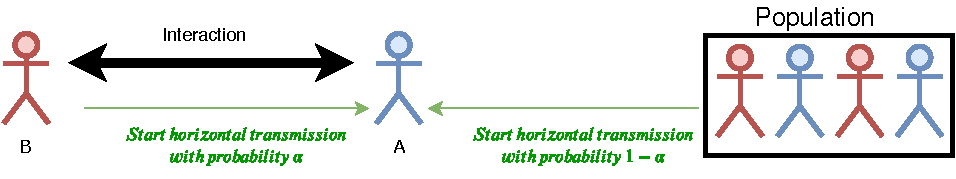
\includegraphics[scale=1]{figure1.pdf}
  \caption{\textbf{Cultural horizontal transmission.} Transmission occurs between interacting partners with probability $\alpha$ (left) or between two random peers with probability $1-\alpha$.}
  \label{fig:horizontal}
\end{figure}

% Results
\section*{Results}

We start by studying specific cases, for which we can derive general results, and then 
we use numerical simulation to analyze more complex cases.

%%%%%%%%%%%%%%%%%%%%%%%%%%%%%%%%%%%%%%%%%%%%%%%%
\subsection*{Without Oblique Transmission}

With only vertical and horizontal transmission, i.e. $v=1$, eq.~\ref{eq:horizontal} becomes
$\hat{p} =  \tilde{p}$,
and eq.~\ref{eq:nextgen_parents_simplified} for the change in frequency $p'$ of phenotype $A$ among parents can be written as

\begin{equation} 
\begin{split}\label{eq:nextgen_parents_vertical_only}
\bar{w} \tilde{p}' 
& = \tilde{p}^2 (1+b-c) [1 - (1-\tilde{p}) (1-\alpha) T_B] \\
& + \tilde{p}(1-\tilde{p}) (1-c) [\tilde{p} (1-\alpha) T_B + 1 - T_B] \\
& + \tilde{p}(1-\tilde{p}) (1+b) [\tilde{p} (1-\alpha) + \alpha] T_A \\
& + (1-\tilde{p})^2 \tilde{p} (1-\alpha) T_A
\end{split}
\end{equation}

We find the following result and corollaries.

\textbf{Result 1: Vertical and horizontal transmission of cooperation.}
From eq.~\ref{eq:nextgen_parents_vertical_only}, if
\begin{equation} \label{eq:unequal_transmission}
c \cdot (1-T_B) < b \cdot  \alpha T_A  + (T_A - T_B) [1 + b\tilde{p}(1-\alpha)] ,
\end{equation}
then $\tilde{p}' > \tilde{p}$, and the frequency of the cooperator phenotype $A$ among parents increases every generation.

\textbf{Corollary 1.1: Symmetric horizontal transmission.}
If $T=T_A=T_B$, then
\begin{equation}
\label{eq:equal_transmission}
c < b \cdot \frac{\alpha T}{1-T},
\end{equation}
which can be seen as a cultural version of \emph{Hamilton's rule} (eq.~\ref{eq:hamilton_rule}), where $r_H=\alpha T/(1-T)$ can be thought of as \emph{horizontal relatedness}.
Therefore, if the cost $c$ is less than the benefit $b$ times the horizontal relatedness $r_H$, then cooperation will take over of the population (see~\textbf{\autoref{fig:results_a}}).

\textbf{Corollary 1.2: Complete correlation between transmission and cooperation.}
	
In this case $\alpha=1$, and horizontal transmission can only occur as a result of cooperative interactions.
Therefore, eq.~\ref{eq:unequal_transmission}, which determines the conditions for evolution of cooperation, becomes
\begin{equation}\label{eq:horizontal_transmission_only_after_interaction}
c \cdot (1-T_B) < b \cdot T_A + (T_A - T_B).
\end{equation}
This is equivalent to a result by~\citet[eq.~1]{lewin2017microbes}.

Eq.~\ref{eq:horizontal_transmission_only_after_interaction} can be written as
\begin{equation} \label{eq:horizontal_transmission_only_after_interaction2}
1 - (1-T_B)(1-c) < T_A \cdot (1+b) ,
\end{equation}
which provides an interesting interpretation for the success of cooperation. 
Consider an interaction between two individuals: a cooperator and a defector.
$(1-T_B)(1-c)$ is the probability that the cooperator remains cooperative and also reproduces. 
Therefore, $1 - (1-T_B)(1-c)$ is the probability that either the cooperator becomes a defector, \emph{or} that it fails to reproduce.
This is the effective cost for cooperation from this interaction.
$T_A\cdot(1+b)$ is the probability that the defector becomes cooperative and reproduces.
This is the effective benefit for cooperation from this interaction.
So, eq.~\ref{eq:horizontal_transmission_only_after_interaction2} means that cooperation can evolve if effective cost is less than the effective benefit.

\textbf{Corollary 1.3: No correlation between transmission and cooperation.}

In this case $\alpha=0$, and horizontal transmission is entirely independent from cooperative interactions.  
Then, eq.~\ref{eq:unequal_transmission} becomes
\begin{equation} \label{eq:horizontal_transmission_from_population}
c\cdot(1-T_B) < b \cdot \tilde{p} \;(T_A-T_B) + (T_A-T_B). 
\end{equation}

Therefore, since all the parameters are  positive, cooperation cannot take over the population (and furthermore will become extinct) if cooperators do not have a horizontal transmission bias, i.e. if $T_A\leq T_B$.
When such a bias does exist, $T_A > T_B$, then cooperation will evolve if $\tilde{p} > \tilde{p}^{*}$, where (see also ~\textbf{\autoref{fig:results_b}})
\begin{equation} 
\begin{split} \label{eq:horizontal_transmission_from_population_equilibrium}
\tilde{p}^{*} & = \frac{c}{b} \cdot \frac{1-T_B}{T_A-T_B} - \frac{1}{b}.
\end{split}
\end{equation}
A sufficient condition for evolution of cooperation is that $\tilde{p}^{*} < 0$, namely
\begin{equation} \label{eq:sufficient_horizontal_transmission_from_population}
c < \frac{T_A-T_B}{1-T_B} .  
\end{equation}


%%%%%%%%%%%%%%%%%%%%%%%%%%%%%%%%%%%%%%%%%%%%%%%%
\subsection*{Without Vertical Transmission}

With only oblique and horizontal transmission, i.e. $v = 0$, eq.~\ref{eq:horizontal} becomes $\hat{p}=p$ and eq.~\ref{eq:nextgen_adults_slimpify} becomes % TODO check this, I changed the ref from nextgen_parents_simplified to nextgen_adults_slimpify
\begin{equation}  \label{eq:nextgen_parents_oblique_only}
p' = p^2 (T_B-T_A) + p (1+T_A-T_B) ,
\end{equation}

which gives the following result.

\textbf{Result 2: Oblique and horizontal transmission of cooperation.} 
If there is a horizontal transmission bias in favor of cooperation, namely
\begin{equation} \label{eq:oblique_only_result}
T_A > T_B, 
\end{equation}
then $p'>p$, and the frequency of the cooperator phenotype among adults increases every generation.
Therefore, cooperation will evolve if the cooperator phenotype has a horizontal transmission bias (see~\textbf{\autoref{fig:results_c}}).

%%%%%%%%%%%%%%%%%%%%%%%%%%%%%%%%%%%%%%%%%%%%%%%%
\subsection*{With Vertical and Oblique Transmission}

In this case $0<v<1$, and the recursion system is more complex.
Therefore, we focus on local, rather than global, stability.
To proceed, we note that 
eq.~\ref{eq:horizontal} can give $\hat{p}'$ as a function of both $p'$ and $\tilde{p}'$,
eq.~\ref{eq:nextgen_adults_slimpify} gives $p'$ as a function of $\hat{p}$, and 
eq.~\ref{eq:nextgen_parents_simplified} gives $\tilde{p}'$ as a function of $\hat{p}$. 
Combining these equations, we find an equation for $\hat{p}'$ as a function of $\hat{p}$.
We then determine the equilibria, which are solutions of $\hat{p}' = \hat{p}$, and analyse their local stability: an equilibrium $\hat{p}^*$ is locally stable when the derivative of $f(\hat{p})$ at the equilibrium is negative, $f'(\hat{p}^*)<0$. %MWF: Define f(\hat p).


We start with the simple case of symmetrical horizontal transmission, $T=T_A=T_B$ and 
%MWF: Write the full recursion.
apply eqs.~\ref{eq:horizontal}, \ref{eq:nextgen_adults_slimpify}, and \ref{eq:nextgen_parents_simplified} to obtain 
\begin{equation} \label{eq:equal_horizontal_transmission}
\begin{aligned}
  %\hat{p}' - \hat{p} = 
  %\hat{p} ^2(-\alpha bvT + cv(1-T)) + \hat{p} (\alpha bvT -cv(1-T)) = 
  f(\hat{p}) &= 
  \bar{w}(\hat{p}' - \hat{p}) = \\
  &\hat{p}(1-\hat{p})\big[\alpha bvT - cv(1-T)\big]. % shorter version
\end{aligned}
\end{equation}

The equilibria are solutions of $f(\hat{p})=0$, or $\hat{p}' = \hat{p}$.
It is easy to verify that fixation of either phenotype, $\hat{p} =  0$ and $\hat{p} = 1$, is an equilibrium.
Since the derivative of $f'(\hat{p}$ is 
\begin{equation}
f'(\hat{p})=(1-2\hat{p})\big[\alpha bvT - cv(1-T)\big],
\end{equation}
then the condition for local stability of $\hat{p}=1$ is
\begin{equation} \label{eq:derivative_of_phattag-phat}
	f'(1) =
% 2\cdot\hat{p} (-\alpha bvT + cv(1-T)) + (\alpha bvT -cv(1-T)).
%	(1- 2\hat{p}) (\alpha bvT - cv(1-T)) \mid_{\hat{p}=1} = 
	-\alpha bvT + cv(1-T) < 0,
\end{equation}
which produces the following result.

\textbf{Result 3: Oblique and vertical transmission with symmetric horizontal transmission.}
If horizontal transmission is symmetric, $T = T_A = T_B$, and if
\begin{equation} \label{eq:oblique_and_vertic_result2}
  %\frac{b}{c}>\frac{1-T}{\alpha T}
	c < b \cdot \frac{\alpha T}{1-T},
\end{equation}
then fixation of the cooperator phenotype $A$ is locally stable.
The same condition was given in Corollary 1.1, Eq.~\ref{eq:equal_transmission}.
% TODO what happens if the condition does not apply? can there be an non-zero stable equilibrium?
\\
\\
We now turn to the general case where $T_A \neq T_B$. We have
\begin{equation} \label{eq:general_case_polynomial}
  f(\hat{p}) = \bar{w}(\hat{p}'-\hat{p}) =
  \beta_1 \hat{p}^3 + \beta_2 \hat{p}^2 + \beta_3 \hat{p},
\end{equation}
where 
\begin{equation} \label{eq:polynomial_coefficients}
\begin{aligned}
\beta_1 &= \big[c(1-v) - b (1-\alpha v)\big] (T_A-T_B) , \\
%\beta_2 &= -[c(1-v) - b(1-\alpha v) +  1](T_A-T_B)-\alpha bv T_A + cv(1-T_B) \\
\beta_2 &= -\beta_1 -\beta_3 ,  \\
\beta_3 &= \alpha bvT_A - cv(1-T_B) + (T_A-T_B) .
\end{aligned}
\end{equation}
Since $f(\hat{p})$ is a cubic polynomial, three equilibria may exist, two of which are
$\hat{p} = 0 $ and $\hat{p} = 1$.
By solving $f(\hat{p})/\big[\hat{p}(1-\hat{p})\big] = \beta_3 -\beta_1 \hat{p} = 0$ we  find the third equilibrium
\begin{equation} \label{eq:oblique_and_vertic_result}
  \hat{p}^* =  
  \frac{\beta_3}{\beta_1}.
  %\frac{\alpha bvT_A - cv(1-T_B) + (T_A-T_B)}
  %     {\big(c(1-v) -b (1-\alpha v)\big) (T_A-T_B)} .
\end{equation}

Note that the sign of the cubic $f(\hat{p})$ at positive (negative) infinity is equal (opposite) to the sign of $\beta_1$. 
If $T_A>T_B$, then 
\begin{equation} \label{eq:beta1}
   \beta_1 %& = [c(1-v) - b (1-\alpha v)] (T_A-T_B) \\
   < [c(1-\alpha v) - b(1-\alpha v)] (T_A-T_B) 
   = (1-\alpha v)(c-b)(T_A-T_B) < 0 ,
 \end{equation}
since $c<b$ and $1>\alpha v$, the sign of the cubic at positive and negative infinity is negative and positive, respectively.
First, if $\beta_3<\beta_1$ then 
$1<\hat{p}^*$ and therefore $f'(0)<0$ and $f'(1)>0$, that is, fixation of the defector phenotype $B$ is the only locally stable legitimate (i.e. between 0 and 1) equilibrium.
Second, if $\beta_1<\beta_3<0$ then 
$0<\hat{p}^*<1$ and therefore $f'(0)<0$ and $f'(1)<0$, that is, both fixations are locally stable and $\hat{p}^*$ separates the domains of attraction.
Third, if $0<\beta_3$ then 
$\hat{p}^*<0$ and therefore $f'(0)>0$ and $f'(1)<0$, that is, fixation of the cooperator phenotype $A$ is the only locally stable legitimate equilibrium.


Similarly, if $T_B>T_A$, then
\begin{equation} \label{eq:beta1_rev}
   \beta_1 %& = -[c(1-v) - b (1-\alpha v)] (T_A-T_B) \\
   > [c(1-\alpha v) - b(1-\alpha v)] (T_A-T_B) 
   = (1-\alpha v)(c-b)(T_A-T_B) > 0,
 \end{equation}
since $c<b$, and $1>\alpha v$. So the sign of the cubic at positive and negative infinity is positive and negative, respectively. 
First, if $\beta_3<0$ then $\hat{p}^*<0$ and therefore $f'(0)<0$ and $f'(1)>0$, that is, fixation of the defector phenotype $A=B$ is the only locally stable legitimate equilibrium.
Second, if $0<\beta_3<\beta_1$ then $0<\hat{p}^*<1$ and therefore $f'(0)>0$ and $f'(1)>0$, that is, both fixations are locally unstable and $\hat{p}^*$ is a stable polymorphic equilibrium.
Third, if $\beta_1<\beta_3$ then $\hat{p}^*>1$ and therefore $f'(0)>0$ and $f'(1)<0$, that is, fixation of the cooperator phenotype $A$ is the only locally stable legitimate equilibrium.

The following result summarizes these findings.

\textbf{Result 4: Oblique and vertical transmission of cooperation with asymmetric horizontal transmission.}
The cultural evolution of a cooperator phenotype will follow one of the following scenarios, depending on the horizontal transmission bias $T_A-T_B$ and the coefficients $\beta_1$ and $\beta_3$:
\begin{enumerate}
\item \emph{Fixation of the cooperative phenotype $A$}, if $T_A>T_B$ and $0<\beta_3$, or $T_A<T_B$ and $\beta_1<\beta_3$.

\item \emph{Fixation of the defector phenotype $B$}, if $T_A>T_B$ and $\beta_1<\beta_3<0$, or $T_A<T_B$ and $\beta_3<0$.

\item \emph{Protected polymorphism, or co-existence of both phenotypes}, if $T_A < T_B$ and $0<\beta_3<\beta_1$.

\item \emph{Fixation of either phenotype depending on initial frequency}, if $T_A>T_B$ and $\beta_3<\beta_1$.

\end{enumerate}

\begin{figure}[H]
  \centering
  \begin{subfigure}{8cm}
    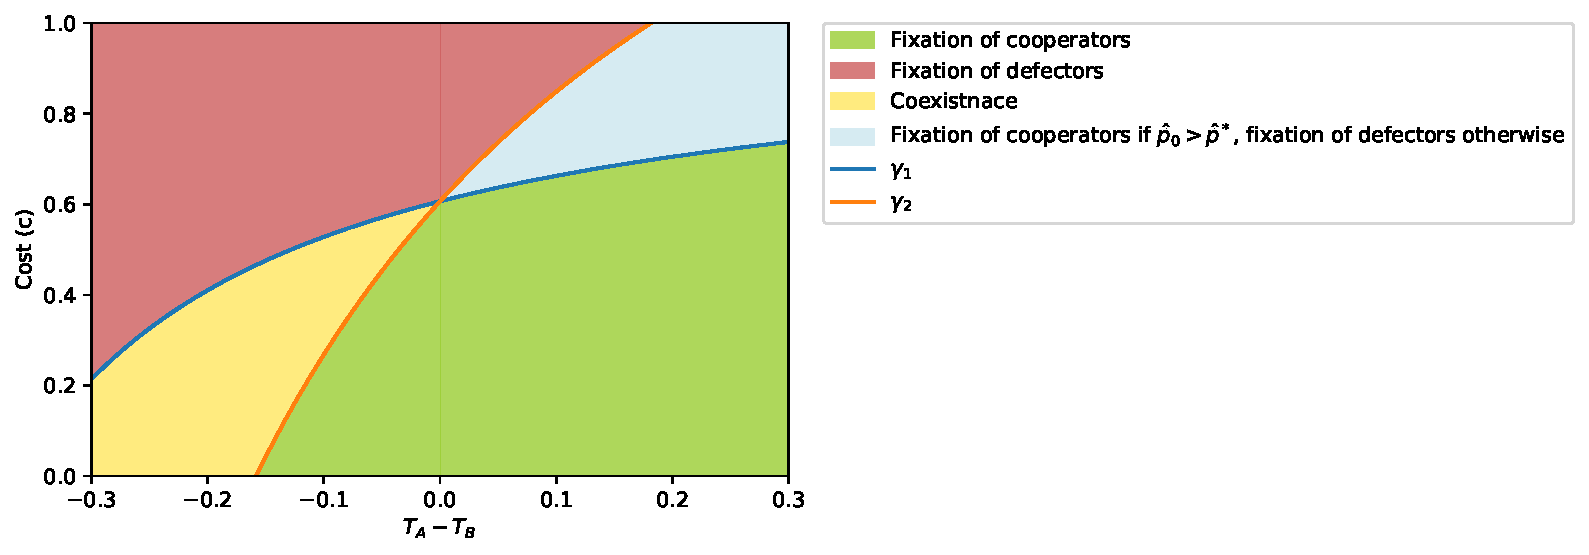
\includegraphics[scale=0.5]{figure2a.pdf}
    \caption{$v=1$, $T_A=T_B=T$, $\alpha \neq 0$}
    \label{fig:results_a}
  \end{subfigure}
  \begin{subfigure}{8cm}
    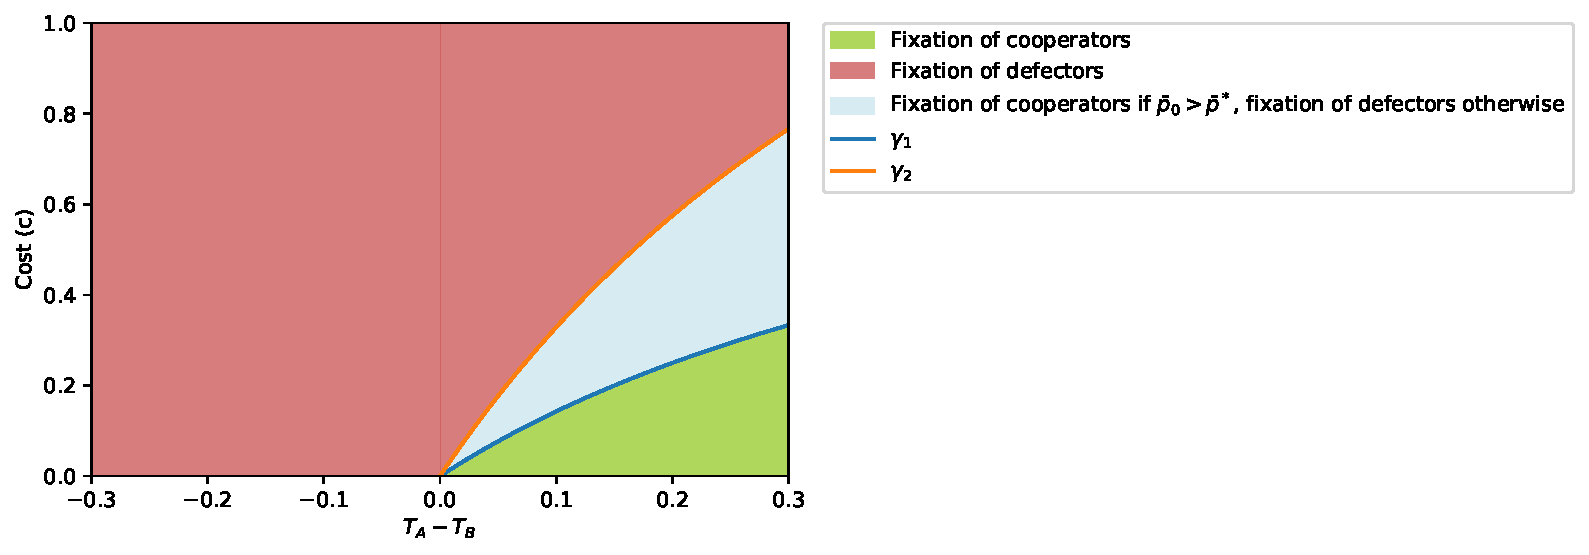
\includegraphics[scale=0.5]{figure2b.pdf}
    \caption{$v=1$, $\alpha = 0$}
    \label{fig:results_b}
  \end{subfigure}
  \begin{subfigure}{8cm}
    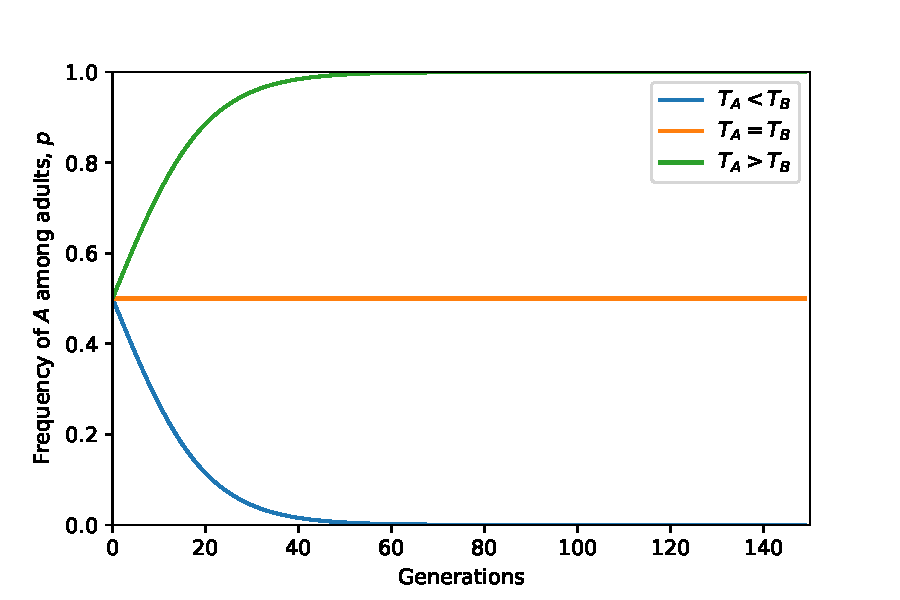
\includegraphics[scale=0.5]{figure2c.pdf}
    \caption{$v=0$}
    \label{fig:results_c}
  \end{subfigure}
  \label{fig:results}
  \caption{
  \textbf{Numerical results for cultural evolution of cooperation.}
  Shown are dynamics of \textbf{(a-b)} $\tilde{p}$, the frequency of parents with cooperative phenotype $A$; \textbf{(c)} $p'$, the frequency of adults with cooperative phenotype $A$.
  The figure demonstrates fixation of cooperation (green), extinction of cooperation (blue)m and stable co-existence of cooperators and defectors (orange).
  %TODO ic (c), the blue and green got mixed. 
  % TODO have all panels in one row.
  }
\end{figure}

% Discussion
%\section*{Discussion}
%We hypothesized that non-vertical transmission can explain the evolution of cooperation. We used a model with non-vertical transmissions and have found that if eq.~\ref{eq:unequal_transmission} is satisfied cooperation will take over the population in fully mixed population with prisoner's dilemma payoff. In addition, we found that when horizontal transmission cannot occur after interaction ($\alpha = 0$) cooperation will always become extinct. 
%Our results improve our understating of cultural evolution of cooperation. Our model shows that cooperation can evolve even in a fully mixed population, where the population is non-structured, there are no repeating interactions and nor individual recognition.

\pagebreak
% Acknowledgements
{\small
\section*{Acknowledgements}
We thank Lilach Hadany and Ayelet Shavit for discussions and comments.
This work was supported in part by
the Israel Science Foundation 552/19 (YR),
and Minerva Center for Lab Evolution (YR).
% TODO funding for other authors?
}

% Bibliography
\bibliographystyle{plainnat}
\bibliography{bib}

% Appendices
\newpage
\section*{Appendix A} % TODO fix equations references
In the section, we start with eq.~\ref{eq:nextgen_parents_vertical_only} and we want to investigate when $\tilde{p}< \tilde{p}'$, that is, when 
\begin{equation} 
\begin{split} \label{eq:horizontal_transmission_from_interaction_step0}
\bar{w}\tilde{p} < & \, \tilde{p}^2 (1+b-c) (1 - (1-\tilde{p}) (1-\alpha) T_B) \\
& + \tilde{p}(1-\tilde{p}) (1-c) (\tilde{p} (1-\alpha) T_B + 1 - T_B) \\
& + \tilde{p}(1-\tilde{p}) (1+b) (\tilde{p} (1-\alpha) + \alpha) T_A \\
& + (1-\tilde{p})^2 \tilde{p} (1-\alpha) T_A
\end{split}
\end{equation}
First divide by $\tilde{p}$ to obtain
\begin{equation} 
\begin{split} \label{eq:horizontal_transmission_from_interaction_step1}
  \bar{w} < & \, \tilde{p}(1+b-c) (1 - (1-\tilde{p}) (1-\alpha) T_B) \\
  & + (1-\tilde{p}) (1-c) (\tilde{p} (1-\alpha) T_B + 1 - T_B) \\
  & + (1-\tilde{p}) (1+b) (\tilde{p} (1-\alpha) + \alpha) T_A \\
  & + (1-\tilde{p})^2 (1-\alpha) T_A
\end{split}
\end{equation}
We know that the mean fitness $\bar{w} = 1 + \tilde{p}(b-c)$ Tthus eq.~\ref{eq:horizontal_transmission_from_interaction_step1} becomes
\begin{equation} 
\begin{split} \label{eq:horizontal_transmission_from_interaction_step2}
  1 + \tilde{p}(b-c) < & \, \tilde{p}(1+b-c) (1 - (1-\tilde{p}) (1-\alpha) T_B) \\
  & + (1-\tilde{p}) (1-c) (\tilde{p} (1-\alpha) T_B + 1 - T_B) \\
  & + (1-\tilde{p}) (1+b) (\tilde{p} (1-\alpha) + \alpha) T_A \\
  & + (1-\tilde{p})^2 (1-\alpha) T_A
\end{split}
\end{equation}
Eq.~\ref{eq:horizontal_transmission_from_interaction_step2} can be simplified to become inequality~\ref{eq:unequal_transmission}.


\end{document}
